\documentclass[conference, onecolumn]{IEEEtran}
\usepackage{hyperref}
\usepackage[utf8]{inputenc}
\usepackage[pdftex]{graphicx}
\usepackage{epstopdf}
\usepackage[plain]{algorithm}
\usepackage{algorithmic}
\usepackage{tabularx}
\usepackage{multirow}
\usepackage{multicol}
\usepackage{amsmath}
\usepackage{amssymb}
\usepackage{longtable}
\usepackage{xspace}
\usepackage{paralist}
\usepackage{listings}
\usepackage{color}
\usepackage{fancyhdr}
\pagestyle{fancy}
\chead{{Bot Filtering and Pertinence Analysis of Tweet Dataset}}
\cfoot{}
\rfoot{\thepage}
\definecolor{mygreen}{rgb}{0,0.6,0}
\definecolor{mygray}{rgb}{0.5,0.5,0.5}
\definecolor{mymauve}{rgb}{0.58,0,0.82}
\lstset{ %
	backgroundcolor=\color{white}, % choose the background color; you must add \usepackage{color} or \usepackage{xcolor}
	basicstyle=\footnotesize, % the size of the fonts that are used for the code
	breakatwhitespace=false, % sets if automatic breaks should only happen at whitespace
	breaklines=true, % sets automatic line breaking
	captionpos=b, % sets the caption-position to bottom
	commentstyle=\color{mygreen}, % comment style
	deletekeywords={...}, % if you want to delete keywords from the given language
	escapeinside={\%*}{*)}, % if you want to add LaTeX within your code
	extendedchars=true, % lets you use non-ASCII characters; for 8-bits encodings only, does not work with UTF-8
	frame=Tb, % adds a frame around the code
	keepspaces=true, % keeps spaces in text, useful for keeping indentation of code (possibly needs columns=flexible)
	keywordstyle=\color{blue}, % keyword style
	language=Octave, % the language of the code
	otherkeywords={*,...}, % if you want to add more keywords to the set
	numbers=left, % where to put the line-numbers; possible values are (none, left, right)
	numbersep=0pt, % how far the line-numbers are from the code
	numberstyle=\tiny\color{mygray}, % the style that is used for the line-numbers
	rulecolor=\color{black}, % if not set, the frame-color may be changed on line-breaks within not-black text (e.g. comments (green here))
	showspaces=false, % show spaces everywhere adding particular underscores; it overrides 'showstringspaces'
	showstringspaces=false, % underline spaces within strings only
	showtabs=false, % show tabs within strings adding particular underscores
	stringstyle=\color{mymauve}, % string literal style
	tabsize=2, % sets default tabsize to 2 spaces
	title=\lstname % show the filename of files included with \lstinputlisting; also try caption instead of title
}

\begin{document}

\title{{Bot Filtering and Pertinence Analysis of Tweet Dataset}}

\author{\IEEEauthorblockN{Federico Migliavacca, Giancarlo Colaci, Luca Cremona}
\IEEEauthorblockA{Dip. Elettronica, Informazione e Bioingegneria - Politecnico di Milano, Italy\\
Email: federico.migliavacca@mail.polimi.it, giancarlo.colaci@mail.polimi.it, luca2.cremona@mail.polimi.it}
}

\maketitle

\begin{abstract}
	This paper presents an experimental analysis for bot searching into a quite big set of data provided. We also analyse the entire set of data to discover similarities beyond tweets using technique well known in literature. The final goal of this work is to search into the filtered dataset to get information about the relevance of tweets to a given topic, by following a set of appropriately chosen keywords.
\end{abstract}

\section{Problem statement}\label{sec:intro}
\medskip
The provided dataset is essentially an .xls file composed of about 180.000 row, we have created a mySql db using this data. We decided to maintain all data in one table as in the Excel file. The table is originally composed by 9 columns:
\begin{itemize}
	\item hosts: describes the author of the tweet;
	\item link: contains the URL of the tweet;
	\item time: date and time of tweet;
	\item auth: number of auth;
	\item follower: number of "followers" of the user; 
	\item following: number of "following" by the user;
	\item country: country of the user;
	\item location: location in which the tweet has been produced;
	\item contents: contains the full text of the tweet;
\end{itemize}
After our manipulation the table in mySql DB contains two extra rows:
\begin{itemize}
	\item mfw\_id: primary key.
	\item pertinenza: represents the result of the work. It will be described later.
\end{itemize}

\section{Bot Filtering and Pertinence Analysis in Literature}\label{sec:literature}
\medskip
Social media ecosystems populated by hundreds of millions of individuals present real incentives to design algorithms that exhibit human-like behaviour. Such ecosystems also raise the bar of the challenge, as they introduce new dimensions to emulate in addition to content, including the social network, temporal activity, diffusion patterns and sentiment expression. 
A social bot is a computer algorithm that automatically produces content and interacts with humans on social media, trying to emulate and possibly alter their behaviour.
One of the greatest challenges for bot detection in social media is in understanding what modern social bots can do.
\medskip

In 2011, James Caverlee's team at Texas A\&M University implemented a honeypot trap that managed to detect thousands of social bots. The idea was simple and effective: the team created a few Twitter accounts (bots) whose role was solely to create nonsensical tweets with gibberish content, in which no human would ever be interested. However, these accounts attracted many followers. Further inspection confirmed that the suspicious followers were indeed social bots trying to grow their social circles by blindly following random accounts.
\medskip

In recent years, Twitter bots have become increasingly sophisticated, making their detection more difficult. The boundary between human-like and bot-like behavior is now fuzzier.
The challenge of social bot detection has been framed by various teams in an adversarial setting. One example of this framework is represented by the Facebook Immune System: an adversary may control multiple social bots (Sybils) to impersonate different identities and launch an attack or infiltration.
\medskip

The possibility of human detection has been explored by Wang et al.  who suggest the crowd-sourcing of social bot detection to legions of workers. As a proof-of-concept, they created an Online Social Turing Test platform. The authors assumed that bot detection is a simple task for humans, whose ability to evaluate conversational nuances like sarcasm or persuasive language, or to observe emerging patterns and anomalies, is yet unparalleled by machines.  The idea of leveraging information about the synchronization of account activities has been fueling many social bot detection systems: frameworks like CopyCatch, SynchroTrap, and the Renren Sybil detector rely explicitly on the identification of such behavior to identify social bots.
\medskip

Released in 2014, "Bot or Not?" was the first social bot detection interface for Twitter to be made publicly available to raise awareness about the presence of social bots. “Bot or Not?” implements a detection algorithm relying upon highly-predictive features which capture a variety of suspicious behaviors and well separate social bots from humans(an example of result is shown in figure \ref{fig:tweetbot}). The system employs off-the-shelf supervised learning algorithms trained with examples of both humans and bots behaviors, based on the Texas A\&M dataset that contains 15 thousand examples of each class and millions of tweets. Bot or Not? scores a detection accuracy above 95,6\% measured by AUROC via cross validation.
\begin{figure} [!htbp]
	\centering
	\vspace{0.3cm}
	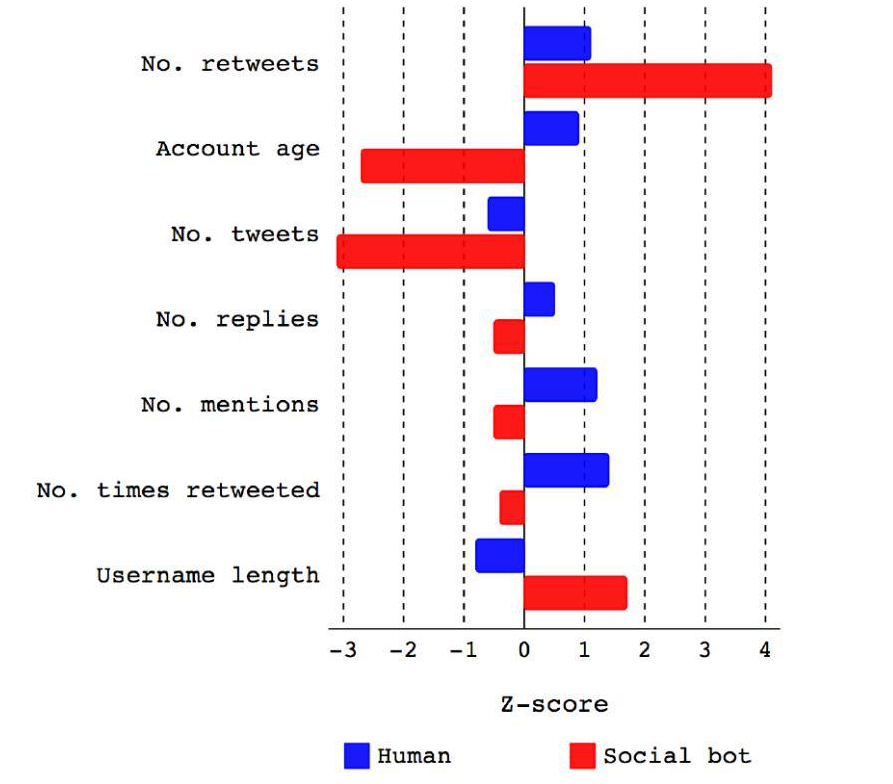
\includegraphics[scale=0.6]{images/tweetbot}
	\caption{Comparison behaviours between human and bot}
	\vspace{0.3cm}
	\label{fig:tweetbot}
\end{figure}
\medskip

Alvisi et al. first recognized the need of adopting complementary detection techniques to effectively deal with Sybil attacks in social networks. The Renren Sybil detector is an example of system that explores multiple dimensions of users' behaviors like activity and timing information. Examination of ground-truth clickstream data shows that real users spend comparatively more time messaging and looking at other users' contents (such as photos and videos), whereas Sybil accounts spend their time harvesting profiles and befriending other accounts. Intuitively, social bot activities tend to be simpler in terms of variety of behavior exhibited.
\medskip

Efforts in the direction of studying platforms vulnerability already started. Some researchers, for example, reverse-engineer social bots reporting alarming results: simple automated mechanisms that produce contents and boost followers yield successful infiltration strategies and increase the social influence of the
bots. Others teams are creating bots themselves: Tim Hwang's and Sune Lehmann's groups continuously challenge our understanding of what strategies effective bots employ, and help quantify the susceptibility of people to their influence. Briscoe et al. studied the deceptive cues of language employed by influence bots. Tools like Bot or Not? Have been made available to the public to shed light on the presence of social bots online.
\medskip

Yet many research questions remain open. For example, nobody knows exactly how many social bots populate social media, or what share of content can be attributed to bots-estimates vary wildly and we might have observed only the tip of the iceberg. These are important questions for the research community to pursue, and initiatives such as DARPA's SMISC bot detection challenge can be effective catalysts of this emerging area of inquiry.

\section{Experimental Analysis}\label{sec:experimental analysis}
\medskip
We can divide our experimental analysis into two parts. The first part mainly covers techniques to eliminate bots while the second attempts to join the difficult problem of detecting the relevance of tweets with respect to a certain topic. To reach both goals we decided to build a set of query.
The queries reported in this paper are also included in a final script that solve the problem for this specific set of data. The script is essentially developed in c++ 2011. The connector for mySql is developed in C. For more information about it and to clone the complete code hosted on GitHub platform follow this link: \url{https://github.com/lucacremona/progettoTIS}
\subsection{Bot Filtering}
\medskip
The problem of bot filtering from a dataset tweet has been analysed using a blacklist approach. The basic idea is to group the tweet by users counting the number of tweets coming from a particular period of time. Following what has already been described extensively in literature, the adoption of a threshold has been necessary. This threshold has been set approximately to 4 tweets per day per user(figure \ref{fig:tweeDay} represent result of a study about " normal number of tweet per day ").
\begin{figure} [!htbp]
	\centering
	\vspace{0.3cm}
	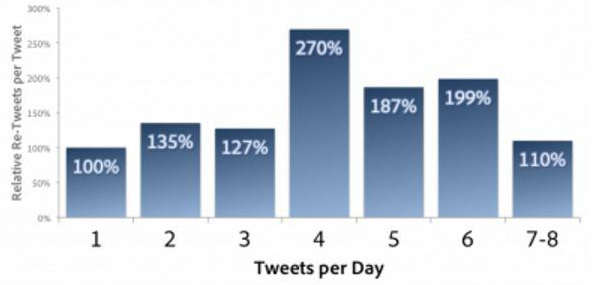
\includegraphics[scale=0.6]{images/daytweet}
	\caption{Retweet by dayly tweet frequency}
	\vspace{0.3cm}
	\label{fig:tweeDay}
\end{figure}
Our specific dataset represents the observation of Twitter platform for one week, during the Milano Fashion Week 2015 event, for this reason we use a global approximate parameter of 30 tweet/week per user. Another parameter that has been taken into account is the number of retweets for each user in a given time interval.The characteristics of the data set provided allow us to set the threshold for the retweet at 15 tweets/week per user.

The following snippet of code represents the queries used to blacklist the bot user.
\begin{lstlisting}
INSERT INTO mfw.mfw_no_bot
					(SELECT * 
					 FROM mfw.mfw 
					 WHERE mfw_id IN
								(SELECT mfw_id
								 FROM mfw.mfw
								 WHERE mfw_id NOT IN
												(SELECT mfw_id
												 FROM mfw.mfw
												 WHERE contents LIKE 'RT @%'
												 GROUP BY host
												 HAVING COUNT(*) > 15
												 )
								GROUP BY host HAVING COUNT(*) < 30
								)
					 )
\end{lstlisting}
\subsection{Pertinence Analysis}
\medskip
For the pertinence analysis we try some techniques based essentially on two metrics: Soundex and Levenshtein.
\begin{itemize}
	\item
	Levenshtein distance:
	In information theory and computer science, the Levenshtein distance is a string metric for measuring the difference between two sequences. Informally, the Levenshtein distance between two words is the minimum number of single-character edits (i.e. insertions, deletions or substitutions) required to change one word into the other. It is named after Vladimir Levenshtein, who considered this distance in 1965.
	Mathematically, the Levenshtein distance between two strings a, b (of length $|a|$ and $|b|$ respectively) is given by $ Lev_{a,b}(|a|,|b|)$ where
	$$Lev_{a,b}(i,j)=\begin{cases} max(i,j), & \mbox{if }min(i,j)=0 \\ min \begin{cases}	Lev_{a,b}(i-1,j)+1, & \\Lev_{a,b}(i,j-1)+1,&\\Lev_{a,b}(i-1,j-1)+1_{(a_i \ne b_j)} & \end{cases} & \mbox{otherwise }	\end{cases}$$
	
	where ${1_{(a_i \ne b_j)}}$ is the indicator function equal to 0 when ${a_i = b_j}$ and equal to 1 otherwise, and $Lev_{a,b}(i,j)$ is the distance between the first $i$ characters of $a$ and the first $j$ characters of $b$.
	Note that the first element in the minimum corresponds to deletion (from  to), the second to insertion and the third to match or mismatch, depending on whether the respective symbols are the same.
	For example, the Levenshtein distance between "kitten" and "sitting" is 3, since the following three edits change one into the other, and there is no way to do it with fewer than three edits:
	\begin{itemize}
	\item kitten $\to$ sitten (substitution of "s" for "k")
	\item sitten $\to$ sittin (substitution of "i" for "e")
	\item sittin $\to$ sitting (insertion of "g" at the end)
	\end{itemize}

	\item Soundex is a phonetic algorithm for indexing names by sound, as pronounced in English. The goal is for homophones to be encoded to the same representation so that they can be matched despite minor differences in spelling. The algorithm mainly encodes consonants; a vowel will not be encoded unless it is the first letter. Soundex is the most widely known of all phonetic algorithms; improvements to Soundex are the basis for many modern phonetic algorithms.
	The Soundex code for a name consists of a letter followed by three numerical digits: the letter is the first letter of the name, and the digits encode the remaining consonants. Consonants at a similar place of articulation share the same digit so, for example, the labial consonants B, F, P, and V are each encoded as the number 1.

	The correct value can be found as follows:
	\begin{itemize}
		\item Retain the first letter of the name and drop all other occurrences of a, e, i, o, u, y, h, w.
		\item Replace consonants with digits as follows (after the first letter):
		\begin{itemize}
			\item b, f, p, v $\to$ 1
			\item c, g, j, k, q, s, x, z $\to$ 2
			\item d, t $\to$ 3
			\item l $\to$ 4
			\item m, n $\to$ 5
			\item r $\to$ 6
		\end{itemize}
		\item If two or more letters with the same number are adjacent in the original name (before step 1), only retain the first letter; also two letters with the same number separated by 'h' or 'w' are coded as a single number, whereas such letters separated by a vowel are coded twice. This rule also applies to the first letter.
		\item If you have too few letters in your word that you can't assign three numbers, append with zeros until there are three numbers. If you have more than 3 letters, just retain the first 3 numbers.
	\end{itemize}
Using this algorithm, both "Robert" and "Rupert" return the same string "R163" while "Rubin" yields "R150".
\end{itemize}
We try to implement both these algorithms in our project but we obtained unexpected results: both them are phonetic, so they can provide a good analysis on how words are pronounced but there are many cases where two words phonetically similar, have opposite, or very different, meanings.
For example, in our case, applying SoundEx to the string "Milan Fashion Week", we found that this string is less similar to "Milan Week Fashion" in spite of "Can't load this page".
For this reason we decided to use a different way to compute the similarity and the pertinence of the tweets. We use some string comparison tools provided by MySql in order to try to match different hash-tags with the same meaning: for example $"\# MilanFashionWeek"$ and $"\# MilanoFashionWeek"$ for us are the same hash-tags. In fact we computed a set of tags pertinent to the argument we treated and also we try to make these "Language Independent" (Italian and English).
\medskip

Once done it we compute the pertinence of every tweet, basing on the string contained in the tweet: we computed five sets, each of them containing string of different level of pertinence and finally we assign to every tweet a class of pertinence.
Results show us that more or less most of tweets not generated by bots are pertinent to the treated theme.
\medskip

The following snippet of code is only an example of query used to filter the tweets with a certain level of pertinence.
\begin{lstlisting}
INSERT IGNORE INTO mfw.mfw_nb_similarity
							(SELECT * , (WEIGHT_SET)
							 FROM mfw.mfw_no_bot
							 WHERE mfw_id IN
										 (SELECT DISTINCT(mfw_id)
										  FROM mfw.mfw_no_bot
										  WHERE(contents LIKE '%#MFW%'
												OR contents LIKE '%fashion%'
												OR contents LIKE '%milan%'
												OR contents LIKE '%Milan Fashion Week%'
												OR contents LIKE '%MFW%'
												OR contents LIKE '%FW%'
												OR contents LIKE '%milan%fashionweek%'
											    )
										  )
							 );
\end{lstlisting}
 The use of IGNORE into query allow us to not overwrite a tweet with a great level of pertinence with one with a lower lever. WEIGHT\_SET is a parameter defined by user that correspond to the level of pertinence for the specific query.
\subsection{Data Validation}
To verify the consistence and the correctness of the produced data, we decided to inspect by hand a set of data before and after the execution of a query. The method adopted is called "Precision and Recall" and consists into:
\begin{itemize}
	\item taking a sample set of records of the database composed by a prefixed, a priori, number of relevant and non relevant information;
	\item applying the same algoritm used for entire dataset;
	\item estimating in percentage the accuracy of data:
	\begin{enumerate}
	\item precision: ratio of the number of relevant records retrieved to the total number of irrelevant and relevant records retrieved
	\item recall: the ratio of the number of relevant records retrieved to the total number of relevant records in the database
\end{enumerate}
\end{itemize}
Having found the relevant tweets with the queries, and so having already a precise method to intercept the records containing the keywords related to the fashion world, we decided to concentrate on the tweets that have been removed from the relevant set. We noticed that from the original database we were able to find 64954 records that are considered created by humans and not by bots. 62873 of these (we can call this number A) have been cataloged in the five categories described above, so the remaining 2081 tweets (C) were marked as irrelevant records. We inspected by hand this set of tweets and we discovered that the number of relevant records not retrieved with the previous method was 3 (B).
The self explicative table show our result with respect to data validation.
\medskip

\begin{tabular}{|c|c|c|}
	\hline & Precision & Recall \\ 
	\hline Formula & A/(A*C) x 100\% & A/(A+B) x 100\% \\ 
	\hline Data & 62873/(62873+3)= 99.995\% & 62873/(62873+2081) = 96.796\% \\ 
	\hline 
\end{tabular}
\medskip

Where A:= number of relevant records retrieved; B:= number of relevant records not retrieved; C:= number of irrelevant records retrieved;

\section{Conclusions}\label{sec:conclusions}
In the Experimental Analysis section we have described essentially which methods we adopt to solve that specific problem. The outputs of our work are two new tables in our database. From the data extract from these new two tables we can do some observations. First, it is easily seen as the elimination of the bot has led to a decrease in lines of about 66\% of the possible tweets. An interesting result that shows that bots detected affect heavily both on the actual amount of data extracted and on the quality and reliability analysis of the data itself. Using the data extracted from the second table it is important to notice that the total amount of tweets are reduced of only 2000 tweets, this is a good index of quality of the pertinence of data provided. An histogram that represents the number of tweets per class is showed in figure \ref{fig:histogram}. We have over 45000 tweets with 100 \% of pertinence with the main topic "Milan Fasion Week 2015" the other classes are very low with respect to the first one. From this result we can conclude that in that specific period of time during the "Milan Fasion Week 2015" people who talk about fashion are talking, in most of the case (80 \% of time), of the main event. This gives immediately the idea of the echo that an event had on social networks.
\medskip

It is important to remember that we decide not to use all column of the table provided because our algorithm does not need it but it can contain some important information about tweets: for example date and time of the tweet could be used to establish how frequently some user or candidate bot create a tweet during a period of time. Another important information that could be used for pertinence in the country of the user and the localization of the user when he/she wrote the tweet. This can also add some useful information about the international or national weight of an event like Milan Fashion Week.
\medskip

In the previous sections we illustrated the proposed algorithms, first to filter the bots from a specific set of data and last to group the tweets about their relevance in the "fashion" context. The first critique that could be moved to these algorithms is a general lack of universality. In fact both algorithms, for similar reasons, require some human intervention before their execution. The "bot filter" algorithm has been calibrated by end, estimating the mean number of tweets per day and consequently the mean number of tweets per week. It is obvious that changing this assumption over the domain, the result can significantly change. The latter algorithm is glaring example of what machine could not, for now, do: as matter of fact the keywords to build the pertinence class have been chosen "by hand" during all work. In a future implementation, this work could be done completely by an algorithm using the power of semantic search. Google Knowledge Graph, the engine at the base of modern software like Google Now, could be integrated to generate keyword for retrieving data with the query. The second critique about that algorithms are linked to the performance. We have built a relational database with only one big table with no specific optimization. Something about index, hash table based for example, could be done. Another future evolution, after the extraction of data, is to try to store the information about their relevance in RDF/graph database to improve next access to the information.
\begin{figure} [!htbp]
	\centering
	\vspace{0.3cm}
	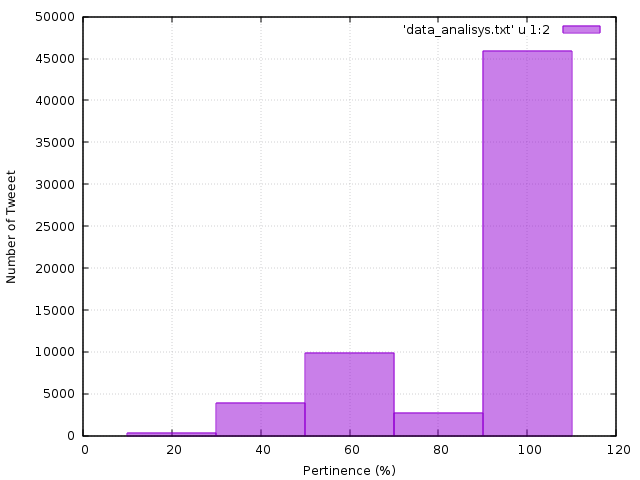
\includegraphics[scale=0.6]{images/hystogram}
	\caption{Histogram of tweet per pertinence class}
	\vspace{0.3cm}
	\label{fig:histogram}
\end{figure}
%\cite{IndianaUniversity}
%\cite{wiki:123}
\bibliographystyle{IEEEtran}
\bibliography{biblio}
\end{document}